\documentclass[8pt,a4paper]{scrartcl}

\usepackage[ngerman]{babel}

\input{../Headerfiles/Packages}
\input{../Headerfiles/Titles}
\input{../Headerfiles/Commands}

\setlength{\columnseprule}{0.5pt}
\renewcommand{\baselinestretch}{1}
\parindent 0pt

\renewcommand{\compaq}{\setlength{\itemsep}{0mm}\setlength{\parskip}{0cm}}

\begin{document}

\setlength{\columnsep}{8mm}
\begin{multicols*}{3}
%%%%%%%%%%%%%%%%%%%%%%%%%

\section{Lagrange and Least Squares}
\subsection{Function Fitting}

Fitting function $f(x) = \sum_{k=1}^M \alpha_k \phi_k (x) $

With possible basis functions:
\begin{tabular}{|ll|}
\hline
$\phi_k (x) = x ^{k-1} $&$\phi_k (x) = \cos [(k-1)x]$\\
$\phi_k (x) = e^{\beta_k x} $&$\phi_k (x) = 1- \frac{|x - x_k|}{\Delta}$\\
\hline
\end{tabular}

\subsection{Linear Interpolation $N = M$}

Problem statement: $f(x_i) = \sum_{k=1}^M \phi_k (x_i) \alpha_k = y_i, \quad i = 1\dots N$

To determine the coefficients, we solve the following system equations:
\begin{equation*}
\Phi \vec \alpha = \vec y
\end{equation*}
\begin{equation*}
\begin{pmatrix}
\phi_1 (x_1)  & \phi_2 (x_1)  & \dots & \phi_M (x_1)  \\
\phi_1 (x_2)  & \phi_2 (x_2)  & \dots & \phi_M (x_2)  \\
\vdots &  &  & \vdots \\
\phi_1 (x_N)  & \phi_2 (x_N)  & \dots & \phi_M (x_N) 
\end{pmatrix}
\begin{pmatrix}
\alpha_1\\
\alpha_2\\
\vdots \\
\alpha_M
\end{pmatrix}
=
\begin{pmatrix}
y_1\\
y_2\\
\vdots \\
y_N
\end{pmatrix}
\end{equation*}

\subsubsection{Lagrange Interpolation}

Idea: Create basis functions such that the matrix above becomes the identity matrix.

\begin{itemize}\compaq

\item Polynomials of same degree as the number of data points
\item Sensitive to noise
\item Predictability issues
\item Passes through all the points
\item Lagrange polynomials form a basis of $P_{N-1}$
\item Choose $x_n$ to be the roots of the Chebychev polynomials.
\end{itemize} 
Construct $N$ polynomials of degree $N-1$: $\{ l_k (x), \; k = 1, \dots, N \}$, such that $l_k (x_i) = \delta_{ki}$.
\important{$l_k(x) = \prod_{\substack{1 \leqslant i \leqslant N \\ i \neq k}} \frac{x - x_i}{x_k - x_i} \quad \rightarrow \quad f(x) = \sum_{k=1}^N y_k l_k(x)$}

\importname{Lagrange in 3D}{$l_k(x,y) = \prod_{\substack{1 \leqslant i \leqslant N \\ i \neq k}} \frac{(x - x_i)^2 + (y-y_i)^2}{(x_k - x_i)^2 + (y_k-y_i)^2}$}

\importname{Error}{$\left|y(x) - f(x)\right| = \left| \frac{y^{(n)}(\xi)}{n!} \Pi_{k=1}^n (x-x_k) \right|, \; x_1 \le \xi \le x_N$}

\subsection{Least Squares $N < M$}

\begin{itemize}\compaq
\item Low order model of data
\item Less sensitive to noise
\item Higher computational complexity
\end{itemize} 
Equation system, $N$ data points, $M$ unknown parameters: $A \vec x = \vec b$

If the system is inconsistent, $\vec{b}\notin\text{span}(A)$. We are looking for $\vec{x}$ which minimizes the error: $E = \|A \vec{x} - \vec b\|$. 
	
\finn

$\rightarrow A\vec{x}-b$ has to be perpendicular to the column space of A: $A\vec{y}$. 

$(A\vec{y})^T(A\vec{x}-b)=0\Rightarrow y^T[A^TA\vec{x}-A^T\vec{b}]=0$

\important{$A^TA\vec{x} = A^T \vec b\qquad\Rightarrow \vec{x}=(A^TA)^{-1}A^Tb$}

\subsubsection{Least Squares Fitting of 3-D Data}

This example can easily be applied to the 2-D data case. \\ \\
Given set of $N$ data $\{x_i,y_i,z_i\}_{i=1}^N$, we wish to fit to a linear function of 3 parameters A, B and C given by:
\begin{equation*}
A + Bx_i + Cy_i \approx z_i  \quad \text{or} \quad
\begin{pmatrix}
1 & x_1 & y_1 \\
1 & x_2 & y_2 \\
\vdots & \vdots & \vdots \\
1 & x_N & y_N
\end{pmatrix}
\begin{pmatrix}
A\\
B\\
C
\end{pmatrix}
\approx
\begin{pmatrix}
z_1 \\
z_2 \\
\vdots \\
z_N
\end{pmatrix}
\end{equation*}
$A^TA\bar{x} = A^T \vec b$ leads to the final system of equation (\hlcyan{2D, $z_i\rightarrow y_i$}):
\begin{equation*}
\begin{pmatrix}
$\hlcyan{$N$}$		& $\hlcyan{$\sum x_i$}$		& \sum y_i\\
$\hlcyan{$\sum x_i$}$	& $\hlcyan{$\sum x_i^2$}$	& \sum x_i y_i\\
\sum y_i	& \sum x_i y_i	& \sum y_i^2
\end{pmatrix}
\begin{pmatrix}
$\hlcyan{$A$}$\\
$\hlcyan{$B$}$\\
C
\end{pmatrix}
=
\begin{pmatrix}
$\hlcyan{$\sum z_i$}$\\
$\hlcyan{$\sum z_i x_i$}$\\
\sum z_i y_i
\end{pmatrix}
\end{equation*}

\subsubsection{The Projection Matrix $P$}

Closest point to $\vec b$ is:
\begin{equation*}
A \bar{x} = \vec p = A(A^TA)^{-1}A^T \vec b \quad \rightarrow \quad P = A(A^TA)^{-1}A^T
\end{equation*}
The matrix $P$ is idemptotent: $P^2 = P$ and symmetric: $P = P^T$.

\note{Orthogonal case: $A^TA=\mathbb{I}$}

\section{Splines}


\subsection{Cubic Splines}

We try to fit a cubic function $f_i(x)$ between two data points with $f_i' = f_{i+1}'$ and $f_i'' = f_{i+1}''$ at each node $\{ x_{i} , y_{i} \}$. $(i=1\cdots N)$

\begin{center}
$2_{nd}$ derivative is a piecewise linear function \dahe integrate twice:

\finn

$f(x) = f_i ''\! \frac{(x_{i+1} -x)^3}{6 \Delta_i} + f_{i+1} '' \frac{(x-x_i)^3}{6 \Delta_i} + C_i(x-x_i) + D_i$

\finn

evaluate at $\{x_i,y_i=f(x_i)\}$ and $\{x_{i+1},y_{i+1}=f(x_{i+1})\}$ to get:

\finn

$C_i=\left( \frac{y_{i+1}-y_i}{\Delta_i} - (f_{i+1}'' - f_i '') \frac{\Delta_i}{6} \right)$\hfill$D_i=\left(y_i-f_i'' \frac{\Delta_i ^2}{6} \right)$
\normalsize
\end{center}

\finn
for \hlcyan{$x_i\leq x\leq x_{i+1}$}: 

$f'(x)=f_{i+1}''\left[\frac{(x-x_i)^2}{2\Delta_i}-\frac{\Delta_i}{6}\right]-f_i''\left[\frac{(x_{i+1}-x)^2}{2\Delta_i}-\frac{\Delta_i}{6}\right]+\frac{y_{i+1}-y_i}{\Delta_i}$

for \hlpink{$x_{i-1}\leq x\leq x_i$}:

$f'(x)=f_i''\left[\frac{(x-x_{i-1})^2}{2\Delta_{i-1}}-\frac{\Delta_{i-1}}{6}\right]-f_{i-1}''\left[\frac{(x_i-x)^2}{2\Delta_{i-1}}-\frac{\Delta_{i-1}}{6}\right]+\frac{y_i-y_{i-1}}{\Delta_{i-1}}$

\finn

With $\Delta_i = x_{i+1} - x_i$, $f''(x_i) = f_i''$ and the condition that $f'(x)$ must be continuous \hlpink{$f'(x_i)$}=\hlcyan{$f'(x_i)$} the equation that must be solved is:
\begin{equation*}
\begin{split}
\frac{\Delta_{i-1}}{6} f_{i-1}'' + (\frac{\Delta_{i-1} + \Delta_i}{3})f_i'' + \frac{\Delta_i}{6}f_{i+1}'' & = \frac{y_{i+1}-y_i}{\Delta_i} - \frac{y_i - y_{i-1}}{\Delta_{i-1}} \\
\Rightarrow \quad A_i f_{i-1}'' + B_i f_i'' + C_i f_{i+1}'' & = D_i
\end{split}
\end{equation*}
Boundary conditions:
\begin{itemize}\compaq
\item Natural spline: $f_1'' = f_N'' = 0$
\item Splines with clamped boundaries: $f_1' = f_N' = 0$
\item Parabolic runout: $f_1'' = f_2''$ and $f_N'' = f_{N-1}''$
\item General equation not valid for end points, except for periodic case
\end{itemize}
Example of system with $N = 4$ and clamped boundaries:
\begin{equation*}
\begin{pmatrix}
B_1 & C_1 & 0 & 0\\
A_2 & B_2 & C_2 & 0\\
0 & A_3 & B_3 & C_3\\
0 & 0 & A_4 & B_4
\end{pmatrix}
\begin{pmatrix}
f_1''\\
f_2''\\
f_3''\\
f_4''
\end{pmatrix}
=
\begin{pmatrix}
D_1\\
D_2\\
D_3\\
D_4
\end{pmatrix}
\end{equation*}

\begin{itemize}\compaq
\item
Goes through all control points.
\item
Only uses lower order polynomials.
\item
Continuous $2_{nd}$ derivative.
\end{itemize}

\subsection{B-splines and NURBS}

General ``B-spline approach'' with free parameters $\alpha_i$ to be determined:
\begin{equation*}
S_{d,t}(x) = \sum_{i=1}^M \alpha_i B_{i,d,t}(x)\qquad \text{\footnotesize Find $\alpha_i$ with linear least squares.\normalsize}
\end{equation*}

\note{N=M forces $S_{d,t}(x)$ to go through all points. Change one point \dahe recompute all coefficients.}

The B-spline $B_{i,d,t}(x)$ is itself constructed as piecewise \hlcyan{polynomials of degree d} which is \hlcyan{only non-zero for the range $t_i \le x \le t_{i+d+1}$.} $N$ data points lead to $N$ splines ($i=1,\dots,N$) with \hlcyan{continuous derivatives up to degree d-1.} The \hlcyan{size of the knot vector $t$ is therefore $N+d+1$.}
\begin{equation*}
B_{i,0,t}(x) =
\begin{cases}
1 & \text{if } t_i \le x \le t_{i+1}\\
0 & \text{otherwise}
\end{cases}
\end{equation*}
\begin{equation*}
B_{i,d,t}(x) = \frac{x-t_i}{t_{i+d}-t_i} B_{i,d-1,t}(x) + \frac{t_{i+d+1}-x}{t_{i+d+1}-t_{i+1}} B_{i+1,d-1,t}(x)
\end{equation*}
%\newpage
%\noindent 
\textbf{NURBS} (Non-Uniform Rational B-Splines)\\ \\
$N$ data points $\vec p_i = \{ x_i,y_i \},  (i = 1,\dots,N)$ each weighted by $w_i$. The curve is parametrized as $\vec p (s) = \{x(s),y(s)\}$ for $t_{d+1} \le s \le t_{N+1}$ as follows:
\begin{equation*}
\vec p(s) = \sum_{i=1}^N R_{i,d,t}(s) \vec p_i  \quad \text{with} \quad R_{i,d,t}(s) = \frac{B_{i,d,t}(s) w_i}{\sum_{j=1}^N B_{j,d,t}(s) w_j}
\end{equation*}
If B-splines with \textbf{``clamped''} knots are used, the curve is guaranted to start at the first control point and end at the final one.
\begin{equation*}
t = \{ \underbrace{t_1,\dots,t_{d+1}}_{\shortstack{d+1 \\ equal knots}}, \underbrace{t_{d+2},\dots,t_N}_{\shortstack{N-d knots}}, \underbrace{t_{N+1},\dots,t_{N+d+1}}_{\shortstack{d+1 \\ equal knots}} \}
\end{equation*}

\note{Interval between two equal nodes is trivial. Does not produce a new spline.}

\subsection{Multivariate Interpolation}

Given $z_k = Z(x_k,y_k)$ for $k = 1,\dots,N$ we must find a reasonable function f(x,y) such that $z_k = f(x_k,y_k)$

\subsubsection{Gridded Data}

In the case of gridded data we can use as functions the tensor products of functions in 1-dimension.
\begin{equation*}
f(x_p,y_q) = Z(x_p,y_q) = \sum_i \sum_j \alpha_{ij} \cdot \phi_i(x_p) \cdot \phi_j(y_q)
\end{equation*}
Using Lagrange polynomials:
\begin{equation*}
f(x_p,y_q) = \sum_i \sum_j Z(x_i,y_j) \cdot l_i(x_p)\cdot  l_j(y_q)
\end{equation*}
Using NURBS surfaces:
We define a ``grid'' of $N \times M$ control points $\vec p_{ij} = \{x_{ij},y_{ij},z_{ij}\}$. The two dimensions of the grid of control points correspond to two parametric dimensions $u$ and $v$. For each parametric dimension we fix the degree to be $d_U$ and $d_V$, and define knot vectors $t_U$ and $t_V$.
\begin{equation*}
\vec p(u,v) = \sum_{i=1}^N \sum_{j=1}^M R_{i,d_U,t_U}(u) \cdot R_{j,d_V,t_V}(v) \cdot \vec p_{ij}
\end{equation*}

%\subsubsection{Irregular Data}
%
%\textbf{Shepard's method:} Optimal method to approximate const. functions:
%\begin{equation*}
%f(x,y) = \frac{\sum_{k=1}^n z_k \cdot g(x-x_k,y-y_k)}{\sum_{k=1}^n g(x-x_k,y-y_k)}
%\end{equation*}
%where the function g(x,y) is usually selected to be a function with radial symmetry and decaying away from the data points. Originally (with $\mu$ being a free parameter):
%\begin{equation*}
%g(x,y) = \frac{1}{(x^2 + y^2)^{\mu/2}}
%\end{equation*}
%\textbf{Coons patch:} Consider a square occupying the area $(0 \le x, y \le 1)$ and the data is given along the edges of the square, that is we know the values at $z(x,0), z(0,y), z(x,1), z(1,y).$ \\
%The method of Coons reads:
%\begin{align*}
%& z(x,y) = \\ 
%& y \cdot z(x,1) +(1-y) \cdot z(x,0) \quad \rightarrow \text{linear interpolation in } y\\
%& + x \cdot z(1,y) + (1-x) \cdot z(0,y) \quad \rightarrow \text{linear interpolation in }x\\
%&-(1-x) \cdot (1-y) \cdot z(0,0) - (1-x) \cdot y \cdot z(0,1) \quad \rightarrow \text{bilinear interp.}\\
%& -(1-y) \cdot x \cdot z(1,0) - x \cdot y \cdot z(1,1) \quad \rightarrow \text{bilinear interp.}
%\end{align*}

\section{Choosing basis functions}


\subsection{Orthogonal Functions}

Definition: $\langle\phi_i\phi_j\rangle=\intinf \phi_i\phi_jdx=\delta_{ij}=\begin{cases}1&i=j\\0 &\text{otherwise}\end{cases}$

Advantage: enable to add additional basis functions without recomputing previous parameters.
Functional representation of $y(x)$ is given by
\begin{equation*}
y(x) = \sum_{i=1}^M \alpha_{i} \phi_{i} (x)
\end{equation*}
with the coefficients $\alpha_i$ and orthonormal basis functions $\phi_i$:
\begin{equation*}
\alpha_i = \int_{-\infty}^{\infty} y(x) \phi_i(x) dx
\end{equation*}
With a set of \textbf{experimental observations} $\{ x_i , y_i \}_{i = 1,\dots,N}$ the basis functions must be orthonormal with respect of the probability density $p(x)$:
\begin{equation*}
p(x) \approx \frac{1}{N} \sum_{n=1}^{N} \delta (x-x_n) \\
\end{equation*}
\begin{equation*}
\rightarrow \langle \phi_{i}(x), \phi_{j}(x) \rangle  = \int_{-\infty}^{\infty} \phi_i(x) \phi_j(x) p(x) dx = \delta_{ij}
\end{equation*}
Which leads to a new formula for computing the coefficients and to the general discrete inner product:
\begin{equation*}
\alpha_i \approx \frac{1}{N} \sum_{n=1}^{N} y_n \phi_i (x_n)
\end{equation*}
\begin{equation*}
\langle f(x), g(x) \rangle = \frac{1}{N} \sum_{i=1}^{N} f(x_i) g(x_i)
\end{equation*}
Possible basis functions:
\begin{itemize}\compaq
\item Hermite polynomials, orthogonal with respect to $e^{-x^2}$
\item Laguerre polynomials, orthogonal with respect to $e^{-x}$
\item Chebyshev polynomials, orthogonal with respect to $(1-x^2)^{-\frac{1}{2}}$
\end{itemize}

\subsubsection{Gram-Schmidt process}

\begin{itemize}
\item Normalize first basis function: $\phi_1 = \frac{g_1}{\langle g_1(x) , g_1(x) \rangle^{1/2}}$
\item Find orthogonal function $\tilde \phi_2$ and normalize it to $\phi_2$

$\tilde \phi_2 = g_2(x) - \phi_1(x) \frac{1}{N} \sum_{n=1}^N \phi_1(x_n) g_2(x_n)$


$\phi_2 = \frac{\tilde \phi_2}{\langle \tilde \phi_2(x) , \tilde \phi_2(x) \rangle^{1/2}} $

\item Find third orthogonal function etc.

\small
$\tilde \phi_3 = g_3(x) -  $\hlyellow{$\phi_1(x)$}$ \frac{1}{N} \sum\limits_{n=1}^N \phi_1(x_n) g_3(x_n) - $\hlyellow{$\phi_2(x)$}$\frac{1}{N} \sum\limits_{n=1}^N \phi_2(x_n) g_3(x_n)$\normalsize

\end{itemize}


\subsection{Radial Basis Functions}

Advantages:
\begin{itemize}
\item Extra terms added without increased divergence (since all basis functions are identical)
\item Centers can be placed where needed
\end{itemize}
We choose a set of identical basis functions $\phi$, which depend on the distance from a set of ``centers'' $c_i$ and on parameters $\alpha_i$:
\begin{equation*}
y(x) = \sum_{i=1}^{N} \phi(|x-c_i|,\alpha_i) \quad \xrightarrow{\text{if linear}} \quad y(x) = \sum_{i=1}^{N} \alpha_i \phi(|x-c_i|)
\end{equation*}
\textbf{Issues:}
\begin{itemize}\compaq
\item Choice of $\phi$, for example:
\begin{align*}
\phi(r) = r \quad   \quad
\phi(r) = r^n \quad  \quad
\phi(r) = e^{-r^2}
\end{align*}
3-D Gaussian RBF:
\begin{equation*}
\phi_i(x,y) = \frac{1}{2\pi \sigma_x \sigma_y}  \text{exp} \left\{ - \frac{1}{2} \left( \frac{(x-c_{xi})^2}{\sigma_x^2} + \frac{(y-c_{yi})^2}{\sigma_y^2} \right) \right\}
\end{equation*}
\item Choice of $c_i$: Randomly, Uniformly or Data based?\\
\item Linear or non-linear coefficients: For non-linear coefficients, iterations are necessary. For linear we need to solve a system as we did for Least Squares. Example:
\begin{equation*}
\begin{pmatrix}
|x_1-c_1|^3  & |x_1-c_2|^3  & \dots & |x_1-c_M|^3  \\
|x_2-c_1|^3  &|x_2-c_2|^3  & \dots & |x_2-c_M|^3  \\
\vdots &  &  & \vdots \\
|x_N-c_1|^3  & |x_N-c_2|^3  & \dots &|x_N-c_M|^3
\end{pmatrix}
\begin{pmatrix}
\alpha_1\\
\alpha_2\\
\vdots \\
\alpha_M
\end{pmatrix}
=
\begin{pmatrix}
y_1\\
y_2\\
\vdots \\
y_N
\end{pmatrix}
\end{equation*}
\end{itemize}

\subsection{Overfitting / Underfitting}

\mypic{Overfitting}

Using too many or too few parameters \dahe we need a method to select the right model \dahe Cross validation.

\subsection{Cross Validation}

\begin{itemize}\compaq
\item Divide the training data $Z = \{ x_i, y_i\}_{i=1,\dots,N}$ to $k$ disjoint samples of roughly equal size $(N/K), Z_1,\dots, Z_K$
\item For each validation sample $Z_i$
\begin{itemize}\compaq
\item Use the remaing data $Z_l = \cup_{j \neq i} Z_i$ to construct an estimate of the model $f_i$
\item For the estimated model $f_i$, average the square errors for the data in $Z_i$:
\begin{equation*}
r_i = \frac{K}{N} \sum_{Z_i} (f_i(x) -y)^2
\end{equation*}
\end{itemize}
\item Compute the estimate for the prediction error by averaging the $r_i$ for $Z_1,\dots,Z_k$
\begin{equation*}
R = \frac{1}{K} \sum_{i=1}^K r_i
\end{equation*}
\end{itemize}

\note{If K=N we do leave one out cross validation.}


\section{Non-Linear Equations}


General approach: 1. Bring the non-linear equation to the form $f(x) = 0$, where $x$ is the unknown parameter. 2. Find the root of $f(\vec x)$.

\subsection{Conditioning for Root finding problems}

If $\frac{1}{|f'(x^\ast|}$ is small, the problem is well conditioned. Thus if $f(\tilde{x})\approx0$, $\tilde{x}$ is sure to be close to $x^\ast$.

\note{$\tilde{x}$ calculated root, $x^\ast$ true root}

\subsection{Convergence rate}

Many schemes proceed by iteratively improving an estimate $x^{(k)}\approx x^\ast$.

Error: $E^{(k)}=x^{(k)}-x^\ast$

Sequence of $x^{(k)}$ converges with rate r if $\quad\lim\limits_{k\rightarrow\infty}\frac{\|E^{(k+1)}\|}{\|E^{(k)}\|^r}=C$

\begin{itemize}\compaq
\item $r=1$: linear
\item $r>1$: superlinear
\item $r=2$: quadratic
\end{itemize}

\subsection{Bisection Method}

The method assumes, when $f(a)$ is negative and $f(b)$ positive, the root of $f(x)$ must be in the range $[a,b]$. With this starting interval $[a,b]$ after $k$ iterations, the interval is $(b-a)/2^k$, so achieving an error tolerance of $tol$ requires $m = \text{log}_2 ((b-a)/tol)$ steps, regardless of $f$.\\ \\
\noindent
\textbf{Algorithm:} Bisection Method
\begin{algorithmic}
\While {$(b-a) > tol$}
\State $m \leftarrow (a+b)/2$
\If {$sign(f(a)) = sign(f(m))$}
\State $a \leftarrow m$
\Else 
\State $b \leftarrow m$
\EndIf
\EndWhile
\end{algorithmic}

\begin{itemize}\compaq
\item Certain to converge but slow.
\item Interval is cut in half every time.
\item Linear convergence (r=1), C=0.5.
\item Achieving error tolerance of tol: steps=$\log_2((b-a)/tol)$.
\end{itemize}

\subsection{Newton's Method}

Take a first guess for $x^{(k)}$ so that $f(x^{(k)})$ is ``somewhere'' around 0. Iterate several times with 
\begin{equation*}
x^{(k+1)} = x^{(k)} - \frac{f(x^{(k)})}{f'(x^{(k)})}\qquad \epsilon_k=\|x_k-x_{k-1}\|
\end{equation*}

\note{simple roots: $(x-1)^1\rightarrow r=2$, higher multiplicity: $(x-1)^2+\rightarrow r=1$}

until $f(x^{(k+1)})$ goes below a certain tolerance. This method is derived by the taylor series $f(x^{(k+1)}) = f(x^{(k)}) + f'(x^{(k)}) (x^{(k+1)}-x^{(k)})$. Since evaluating the derivation may be expensive or inconvenient, we can replace it with a finite difference approximation, the \textbf{Secant Method}.
\begin{equation*}
f'(x^{(k)}) = \frac{ f(x^{(k)}) - f(x^{(k-1)})}{x^{(k)} - x^{(k-1)}}\qquad r=1.618
\end{equation*}

\subsubsection{Solving systems of non-linear equations}

\begin{equation*}
\vec F( \vec x) =
\begin{pmatrix}
f_1(\vec x) \\
\vdots \\
f_N(\vec x) \\
\end{pmatrix}
=
\begin{pmatrix}
0\\
\vdots \\
0
\end{pmatrix}
= \vec 0
\end{equation*}
The derivation $f'(x)$ is replaced by the Jacobian matrix $J$ which is a $N \times N$ matrix with elements $J(\vec x)_{ij} = \partial f_i(\vec x) / \partial x_j$
\begin{equation*}
J(\vec x) = 
\begin{pmatrix}
\frac{\partial f_1}{\partial x_1}(\vec x)  & \dots & \frac{\partial f_1}{\partial x_N}(\vec x)\\
\vdots & \ddots & \vdots\\
\frac{\partial f_N}{\partial x_1}(\vec x) & \dots & \frac{\partial f_N}{\partial x_N}(\vec x)\\
\end{pmatrix}
\end{equation*}
So for the iteration process we get the equation:
\begin{equation*}
\vec x^{(k+1)} = \vec x^{(k)} - J^{-1}(\vec x^{(k)})\vec F (\vec x^{(k)})
\end{equation*}
For not computing the inverse of $J$ we can solve
\begin{equation*}
J(\vec x^{(k)}) \vec y^k = - \vec F (\vec x^{(k)}) \quad \xrightarrow{\text{update}} \quad \vec x^{(k+1)} = \vec x^{(k)} + \vec y^k
\end{equation*}
\noindent
\textbf{Algorithm:} Newton's Method\\
\begin{algorithmic}
\State \textbf{Input:}
\State $\vec x^{(0)}$, \{vector of length N with initial approximation\}
\State $tol$, \{tolerance: stop if $\|\vec x^{(k)} - \vec x^{(k-1)}\| < tol$ \}
\State $k_{max}$, \{maximal number of iterations: stop if $k > k_{max}$\}
\State \textbf{Output:}
\State $\vec x^{(k)}$, \{solution of $\vec F(x^{(k)}) = \vec 0$ within tolerance $tol$\}
\State \textbf{Steps:}
\State $k \leftarrow 1$
\While {$k \leq k_{max}$}
\State Calculate $\vec F(\vec x^{(k-1)})$ and $N \times N$ matrix $J(\vec x^{(k-1)})$
\State Solve the $N \times N$ linear system $J(\vec x^{(k-1)}) \vec y =  - \vec F (\vec x^{(k-1)}) $
\State $x^{(k)} \leftarrow \vec x^{(k-1)} + \vec y$
\If {$\| \vec y \| < tol$}
\State \textbf{break}
\EndIf
\State $k \leftarrow k + 1$
\EndWhile
\end{algorithmic}

\subsubsection{Simplifications to reduce cost}

\begin{itemize}
\item \textbf{Modified Newton Method:} Compute $J^{(0)} = J(x^{(0)})$ only once and solve $J^{(0)} \vec y^k = - \vec F (\vec x^{(k)})$. This method can only succeed if $J$ is not changing rapidly.
\item \textbf{Quasi Newton Method:} $J$ gets updated by using information from the steps. After the first step we know: $\Delta \vec x = \vec x^{(1)} - \vec x^{(0)}$ and $\Delta \vec F = \vec F (\vec x^{(1)}) - \vec F (\vec x^{(0)})$. So derivatives of the $f_i$ are in the direction of $\Delta \vec x$. Then the next $J^{(1)}$ is adjusted to satisfy:
\end{itemize}

\begin{equation*}
J^{(1)} \Delta \vec x = \Delta \vec F
\end{equation*}

\begin{equation*}
J^{(1)} = J^{(0)} + \frac{(\Delta \vec F - J^{(0)} \Delta \vec x)(\Delta \vec x)^T}{(\Delta \vec x )^T (\Delta \vec x )}
\end{equation*}


\section{Numerical Integration}

\note{If integral cannot be solved analytically, the function is known as a set of points.}

\begin{equation*}
I = \int_a^b f(x) dx \quad = \sum_{i=0}^{N-1} \int_{x_i}^{x_{i+1}} f(x) dx \quad \approx \sum_{i=0}^{N-1} I_i
\end{equation*}

\begin{center}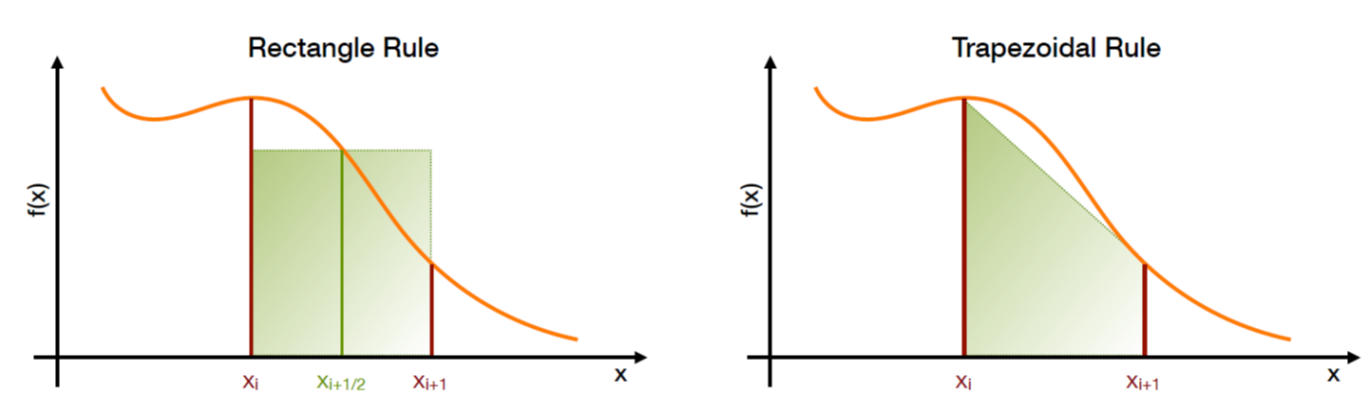
\includegraphics[width=0.9\linewidth]{RectangleTrapezoidalRule}\end{center}

\textbf{Rectangle Rule:}\hfill \note{Uses 2 intervals}
\begin{equation*}
I_{R_i} = f(\frac{x_i + x_{i+1}}{2}) \Delta_i \quad \text{with } \Delta_i = x_{i+1} - x_i
\end{equation*}

\textbf{Trapezoidal Rule:}
\begin{equation*}
I_{T_i} = \frac{f(x_i) + f(x_{i+1})}{2} \Delta_i 
\end{equation*}
\textbf{Simpson's Rule:}\hfill \note{Uses 2 intervals}
\begin{equation*}
I_{S_i} = \frac{f(x_i) + 4f(\frac{x_i + x_{i+1}}{2}) + f(x_{i+1})}{6} \Delta_i 
\end{equation*}
With constant $\Delta_x$ all three formulas can be written as a weighted sum of $f_i$: $I \approx \sum_{i=0}^{N} w_i f_i$.
\begin{align*}
I_R&\approx 2\Delta_x\sum_{\substack{i=1\\i=\text{odd}}}^{N-1} f_i\qquad I_T \approx \frac{\Delta_x}{2} \left( f_0 + 2 \sum_{i=1}^{N-1} f_i + f_N \right) \\
I_S &\approx \frac{\Delta_x}{3} \left( f_0 + 4 \sum_{\substack{i=1\\i=\text{odd}}}^{N-1} f_i + 2 \sum_{\substack{i=1\\i=\text{even}}}^{N-2} f_i + f_N \right)
\end{align*}
\textbf{Newton-Cotes formulas:} approximate the function using Lagrange polynomials, with n + 1 equidistant points in $[a,b]$
\begin{equation*}
I \approx (b-a) \sum_{k=0}^{n} C_k^n f(x_k) \quad \text{with } C_k^n = \frac{1}{b-a} \int_a^b l_k^n(x) dx
\end{equation*}

\importname{Properties of $C_k^n$}{\hlpink{$\sum_{k=0}^n C_k^n = 1 \quad \quad C_k^n = C_{n-k}^n$}}


\note{Because Lagrange polynomials fit $f(x)=1$ perfectly \dahe $\frac{I}{(b-a)}=1=\sum C_k\cdot 1$

for n=2 we get Simpsons rule}

\subsection{Error analysis}

Taylor's series around $x_{i+0.5}$:

$f(x) = f(x_{i+0.5}) + (x - x_{i+0.5})f'(x_{i+0.5}) + \frac{1}{2}(x-x_{i+0.5})^2 f''(x_{i+0.5})+ \frac{1}{6} (x-x_{i+0.5})^3 f''' (x_{i+0.5}) + \dots$

$I_i=\int_{x_i}^{x_{i+1}}f(x)dx=\underbrace{f(x_{i+1/2})\Delta_i}_{I_{R_i}}+\underbrace{0+\frac{1}{24}f''(x_{i+1/2})\Delta_i^3+0+O(\Delta_i^5)}_{\text{error of rectangle rule}}$

$I_{T_i}=\frac{f(x_i)+f(x_{i+1}}{2}\Delta_i=\Delta_i\left(f(x_{i+1/2})+\frac{1}{8}f''(x_{i+1/2})\Delta_i^2+\cdots\right)$

\finn

When we consider the entire Taylor series in our scheme of integration, we can evaluate the error for the different methods:

\small
\begin{align*}
I_{R_i} &= I_i - \frac{1}{24} f''(x_{i+0.5}) \Delta_i^3 + \mathcal{O}(\Delta_i^5) + \dots \\
I_{T_i} &= I_i + \frac{1}{12} f''(x_{i+0.5}) \Delta_i^3 + \mathcal{O}(\Delta_i^5) + \dots \\
I_{S_i} &= \frac{2}{3} I_{R_i} + \frac{1}{3} I_{T_i} = I_i + \mathcal{O}(\Delta_i^5) + \dots
\end{align*}
\normalsize

For the whole domain:\hfill \note{where $N=(b-a)/\Delta_x$}
\begin{align*}
\sum\limits_{i=0}^{N-1}I_{Ri}&=\sum\limits_{i=0}^{N-1}\left(I_i-\frac{1}{24}f''(x_{i+1/2})\Delta_x^3+O(\Delta_x^5)+\cdots\right)\\
\left|\sum\limits_{i=0}^{N-1}I_{Ri}-I\right|&<N\frac{1}{24}\underset{i}{\max}\left(|f''(x_{i+1/2})|\right)\Delta_x^3+NO(\Delta_x^5)+\cdots\\
&=\frac{b-a}{24}\underset{i}{\max}\left(|f''(x_{i+1/2})|\right)\Delta_x^2+O(\Delta_x^4)+\cdots
\end{align*}


\subsection{Richardson Extrapolation and Error Estimation}

Suppose we have a method of approximating a quantity $G$. The approximations depend on a parameter $h$ so that we write $G \approx G(h)$, which can be expressed in terms of a Taylor series for $h$:
\begin{align*}
G(h) &= G + c_1 h + c_2 h^2 + \dots\\
G(h/2) &= G + \frac{1}{2} c_1 h + \frac{1}{4} c_2 h^2 + \dots \\
\Rightarrow G_1(h) &= 2 G(h/2) - G(h) = G + c_2' h^2 + c_3' h^3 + \dots
\end{align*}
In general: $G_n(h) = \frac{1}{2^n -1} \left( 2^n G_{n-1}(h/2) - G_{n-1}(h) \right) = G + \mathcal{O}(h^{n+1})$

\finn

\begin{tabular}{rl}
$\epsilon(h/2)=G(0)-G(h/2)=$&$-\frac{1}{2}c_1h-\frac{1}{4}c_2h^2+O(h^3)$\\
this is similar to $G(h/2)-G(h)=$&$-\frac{1}{2}c_1h-\frac{3}{4}c_2h^2+O(h^3)$
\end{tabular}

\dahe to $1_{st}$ order $\epsilon(h/2)\approx G(h/2)-G(h)$

\finn

If $h$ is small, this will be a good estimate of the error. If the error is not small enough, then this tells the user to keep subdividing.

\subsection{Romberg integration}

Improve inaccurate integration methods by using Richardson's extrapolation. Using a set of trapezoidal approximations $I_0^n$ for $n = 1,2,4,8,\dots$ ($n$ intervals), the method goes as follows:
\begin{equation*}
I_0^n = \frac{b-a}{2n} \left( f(a) + f(b) + 2 \sum_{j=1}^{n-1} f\left(a+j \frac{b-a}{n}\right) \right)
\end{equation*}
Then we recursively calculate the higher order approximations according to the following expression:
\begin{equation*}
I_k^n = \frac{4^k I_{k-1}^{2n} - I_{k-1}^n}{4^k - 1}
\end{equation*}
\note{
\textbf{Note: 1.} How many initial integrals $I_0^k$ we need, depends on the accuracy we want to obtain. If we want to drop the first order $O(h^2)$ term for instance, we only have to compute two initial approximations $I_0^1$ and $I_0^2$. \\
\textbf{2.} The function values of $f(x)$ must not be recomputed in every step. Think of the highest $n$ you will need and calculate all values for this particular case. Then store them for the next computations of $I_0^{n_{\text{max}}/2}, I_0^{n_{\text{max}}/4},\dots,I_0^{1} $.
\textbf{3.} Every iteration the accuracy increases by a factor of 2.
}


\subsection{Adaptive Quadrature}

\textbf{Algorithm:} Adaptive integration\\
\begin{algorithmic}
\State Subdivide the interval of the integration into sub-intervals
\ForAll {sub-intervals}
\State Compute sub-integral, estimate the error (Richardson)
\If {accuracy is worse than desired}
\State Subdivide the interval
\Else
\State Leave the interval untouched
\EndIf
\EndFor
\end{algorithmic}
\noindent
\textbf{Algorithm:} Adaptive integration using recursion and Simpson\\
\begin{algorithmic}
\Function {adaptiveSimpson}{$a,b$}
\State apply Simson's rule in interval $[a,b]$
\State subdivide the interval into $[a,m]$ and $[m,b]$ with $m = (a+b)/2$
\State apply Simpson's rule in intervals $[a,m]$ and $[m,b]$
\State estimate error in $[a,b]$ using Richardson's extrapolation 
\If {accuracy is worse than desired}
\State\Return{\Call{adaptiveSimpson}{$a,m$} + \Call{adaptiveSimpson}{$m,b$} } 
\Else
\State\Return value of Simpson's rule (the accurate one)
\EndIf
\EndFunction
\end{algorithmic}

\subsection{Hermite Interpolation}

Enhancement of Lagrance polynomials \dahe interpolate derivative too.

Given $y_i,y_i'$ find $f(x)$ such that $f(x_i)=y_i$ and $f'(x_i)=y_i'$.

$f(x)=\sum\limits_{k=1}^nU_K(x)\cdot y_k+\sum\limits_{k=1}^nV_k(x)y_k'=H_I(x)$

requiered: \begin{tabular}{l@{$\quad$}l}$U_k(x_j)=\delta_{jk}$&$U_k'(x_j)=0$\\$V_k(x_j)=0$&$V_k'(x_j)=\delta_{jk}$\end{tabular}

solution: \begin{tabular}{ll}$U_k(x)=$&$[1-2L_k'(x_k)(x-x_k)]L_k^2(x)$\\$V_k(x)=$&$(x-x_k)L_k^2(x)$\end{tabular}

\subsection{Gauss Quadrature}

\note{Good for smooth functions, if integrand is non-smooth divide in smooth parts.

Optimal integration points \dahe high accuracy}

Method of indeterminate coefficients: $\int_a^bf(x)dx\approx \sum \omega_i f(x_i)$

Thus n abscissas and n weights adjustable. Polynomials of degree $2n-1$ should be exactly integrable. How to find those?

\begin{itemize}\compaq
\item Change the boundary of the integral: $z = \frac{2x}{b-a} + 1 - \frac{2b}{b-a}$.
\item If $z_i$ and $\omega_i$ given proceed with:
\important{$I \approx \frac{b-a}{2} \sum_{i=1}^n w_i  f\left(\frac{b-a}{2} (z_i-1) + b\right)$}
otherwise they are found as follows (proof):
\item $\int_{-1}^1f(x)dx=\int_{-1}^1H_I(x)\omega(x)dx=\sum\limits_{k=1}^nu_kf(x_k)+\sum\limits_{k=1}^nv_kf'(x_k)$
\note{$u_k=\int_{-1}^1\omega(x)U_k(x)dx\qquad v_k=\int_{-1}^1\omega(x)V_k(x)dx$}
\item $v_k\overset{!}{=}0$ to get the form $I=\int_{-1}^1f(x)dx=\sum\limits_{i=1}^n\omega_if(x_i)$ otherwise $y_i'$ which are generally unavailable would be needed.
\item $L_k=\frac{C_kF(x)}{(x-x_k)}\rightarrow v_k=C_k\int_{-1}^1F(x)L_kdx=0$

\note{$C_k=\prod\limits_{i=1}^n\frac{1}{(x_i-x_k)}\qquad F(x)=\prod\limits_{i=1}^n(x-x_i)$}

Therefore F(x) must be orthogonal to any $L_k$. The only solution to that is given by the Legendre polynomials $P_n(x)$.

\importname{Orthogonality}{$\int_{-1}^1P_n(x)P_m(x)dx=\frac{2}{2n+1}\delta_{nm}$}

\item $x_k$ are the zeros of $P_n(x)$. $u_k=\frac{2}{(1-x_k^2)(P_n'(x_k))^2}$

\note{$u_k$ are symmetric, since $x_k$ are symmetric to the y-axis and $P_n(x),P_n'(x)$ have either even or odd symmetry.}

\item Error with n abscissas: $\epsilon=\frac{2^{2n+1}(n!)^4}{(2n+1)(2n!)^3}f^{(2n)}(\xi)$
\end{itemize}

\subsubsection{Curse of dimensionality}

If we increase the dimensions of our integral, the order of accuracy decreases. Example with Simpson's rule where we have $n$ quadrature points and $d$ dimensions (leading to $M = n^d$ function evaluations):
\begin{align*}
&\text{One dimension ($d=1, M=n$): } & I -I_s = \mathcal{O}(\Delta x^4) \\
&\text{d dimensions: } & I - I_s = \mathcal{O}(M^{-4/d})
\end{align*}

\subsubsection{2 Point Gauss-rule}

\note{Exact result for $3_{rd}$ order polynomial.}

The method of indeterminate coefficients can be used to compute the integral of a 2n-1 polynomial: $f(x)=a_0+a_1x+a_2x^2+a_3x^3$ with $\int_a^bf(x) dx\approx c_1f(x_1)+c_2f(x_2)$.

Comparing the coefficients of $a_i$ leads to the 2 point Gauss-rule:

$\int_a^b{f(x)}dx\approx$

$\frac{b-a}{2}f\left(\left(\frac{b-a}{2}\right)\left(-\frac{1}{\sqrt{3}}\right)+\frac{b+a}{2}\right)+\frac{b-a}{2}f\left(\left(\frac{b-a}{2}\right)\left(\frac{1}{\sqrt{3}}\right)+\frac{b+a}{2}\right)$

\subsection{Monte Carlo Quadrature}

The integral $I$ is defined as follows, with $M$ points $x_i$ (samples) chosen randomly in $\Omega$.
\begin{equation*}
I = | \Omega | \langle f \rangle
\end{equation*}
\begin{equation*}
\text{with } \langle f \rangle = \frac{1}{| \Omega |} \int_{\Omega} f( \vec x) d\vec x \text{ and }  | \Omega | = \int_{\Omega} 1 d \vec x
\end{equation*}
\begin{equation*}
\langle f \rangle \approx \langle f \rangle_M = \frac{1}{M} \sum_{i=1}^{M} f(x_i)
\end{equation*}
\textbf{Error estimation:} \hlyellow{The error does not depend on dimension $d$}
\begin{equation*}
\epsilon_M = \sqrt{\text{Var}[ \langle f \rangle_M - \langle f \rangle]} = \sqrt{\frac{\text{Var}[f]}{M}} = \mathcal{O}(M^{-1/2})
\end{equation*}
\begin{equation*}
\text{Var}[X] = \langle X^2 \rangle - \langle X \rangle^2 = \langle ( X- \langle X \rangle )^2 \rangle
\end{equation*}
\begin{equation*}
| \langle f \rangle - \langle f \rangle_M | < 
\begin{cases}
\epsilon_M, & \text{with probability of } 68\% \\
2\epsilon_M, & \text{with probability of } 95\% \\
3\epsilon_M, & \text{with probability of } 99\% 
\end{cases}
\end{equation*}
Remark: To reduce error by factor $n$, one needs $n^2$ more samples.\\

\textbf{Monte Carlo recipe}

\begin{itemize}\compaq
\item Draw random points $x_i$ and evaluate the integrand $f$ to get random variables $f(x_i)$
\item Store the number of samples $M$, the sum of values, and the sum of squares
\item Compute the mean as the estimate of the expectation (normalized integral) $\langle f \rangle_M$
\item Estimate the variance from the mean of squares and the error
\begin{equation*}
\text{Var}_M[f] = \frac{M}{M-1} \left( \langle f^2 \rangle_M - \langle f \rangle_M^2 \right) \quad \rightarrow \quad \epsilon_M \approx \sqrt{\frac{\text{Var}_M [f]}{M}}
\end{equation*}
\end{itemize}



\end{multicols*}
\end{document}
